\documentclass[10pt]{article}
\usepackage[utf8]{inputenc}
\usepackage[english]{babel}

\usepackage[margin=1in]{geometry} 

\usepackage{amsmath,amsthm,amssymb,amsfonts, bm}
\usepackage{graphicx}
\usepackage{xcolor}

\definecolor{LightGray}{gray}{0.95}
\definecolor{DarkGray}{gray}{0.1}

\usepackage{minted} % code listing
\usemintedstyle{trac}

\newcommand{\code}[1]{{\small\colorbox{LightGray}{\texttt{#1}}}}
\newcommand{\boxx}[1]{{\LARGE\colorbox{LightGray}{\code{#1}}|}}

\setlength{\parindent}{0pt}

\title{Map, hash table and skip list}
\date{}

\begin{document}

\maketitle

\section{Maps and dictionary}
\label{section:map}
A dictionary or map is a collection of pairs \emph{(key, values)} that is searchable. The main operations of a map are inserting an item, deleting an item, and finding an item. The map do not allow for multiple items to have the same key. Given a map $M$ it is possible to access the value of the item with key $k$ with $M[k]$. We can insert an item using $M[k]=v$. We can delete an item with \code{del M[k]}. \code{len(M)} return the number of items in the dictionary. The default iteration \code{\_\_iter\_\_} for a map generate the sequences of \textit{keys} of the map, i.e. it is equivalent to \code{for k in M}. \code{k in M} return True if the key is in the map. \code{M.get(k, d=None)} return the value corresponding to key $k$ if it exist else it returns None. \code{M.setdefault(k, d)} return \code{M[k]} if it exist else set \code{M[k]=d} and return \code{d}. \code{M.pop(k, d)} remove the item with key \code{k} and return its value; if $k\notin M$ return $d$ or raise a \code{KeyError} if $d$ is None. \code{M.popitem()} remove an arbitrary pair $(k, v)$ from $M$ and return it. \code{M.clear} empty the map. \code{M.keys()} and \code{M.values()} return respectively the set of keys and the set of values in the map. \code{M.items()} return a set of pairs in the map. \code{M.update(D)} will set \code{M[k]=v} for each pair $(k, v)\in D$. \code{M1==M2} return \code{True} if all \code{M1} and \code{M2} have identical pair-value associations.\\

\textbf{MutableMapping abstract base class.} The class \code{MutableMapping} provide a concrete implementation of all the method describe in above except for the methods \code{\_\_getitem\_\_}, \code{\_\_setitem\_\_}, \code{\_\_iter\_\_}, \code{\_\_len\_\_}, and \code{\_\_delitem\_\_}. This means that a class that inherit from \code{MutableMapping} should implement these methods, else a \textit{NotImplementedError} should be raise. \\

\textbf{The Map class.} Before implementing the class we need an \code{\_Item} to represent the objects in the map.
\begin{minted}[bgcolor=LightGray]{python}
class Item:
    def __init__(self, key, value=None):
        self._key = key
        self._value = value
     
    def key(self):
        return self._key
        
    def value(self):
        return self._value
\end{minted}
Now we can implement the class Map. The class Map needs a \code{is\_empty()} method that return True if the map is empty, a \code{get($k$)} method that return the value corresponding to kek $k$, and a \code{setdefault($k$, $d$)} method that returns the value corresponding to the key $k$ if it is in the map, else it set \code{M[$k$]=$d$} and return $d$. 
\begin{minted}[bgcolor=LightGray]{python}
class Map(MutableMapping, Item):
    def is_empty(self):
        return len(self) == 0
    
    def get(self, k, d=None):
        try:
            return self[k]
        except KeyError:
            return d
            
    def setdefault(self, k, d=None):
        if self.get(k) is not None:
            return self.get(k)
        else:
            self[k] = d
            return d
\end{minted}
\subsection{Implementing Map with a list.}
We can implement Map with an unsorted list. We stock the element of a Map is a list $S$ in an arbitrary order. We need to implement 7 methods for the class Map: \code{\_\_setitem\_\_} set a key to a particular value and return nothing, \code{\_\_getitem\_\_}, \code{\_\_len\_\_}, \code{\_\_iter\_\_} that provide an iterator on the keys, \code{\_\_items\_\_} that provide an iterator on the items, \code{\_\_contains\_\_}, and \code{\_\_delitem\_\_}. 
\begin{minted}[bgcolor=LightGray]{python}
class ListMap:
    def __init__(self):
        self._T = []
        
    def __getitem__(self, k):
        for item in self._T:
            if k == item._key:
                return item._values
        raise KeyError(k)
        
    def __setitem__(self, k, v):
        for item in self._T:
            if k == item._key:
                item._value = v
                return
        self._T.append(Item(k, v))
    
    def __len__(self):
        return len(self._T)
        
    def __contains__(self, k)
        try: 
            self[k]
        except KeyError:
            return False
        return True
    
    def __iter__(self):
        for item in self._T:
            yield item.key()
    
    def __items__(self):
        for item in self._T:
            yield (item.key(), item.value())
    
    def __delitem__(self, k):
        for i, item in enumerate(self._T):
            if k == item.key():
                self._T.pop(i)
                return
        raise KeyError(k)
        
\end{minted}

\textbf{Performance of the Map implementation with an unsorted list} Inserting can be done in $O(1)$ since we can insert an item at the end of the list using \code{append}, but because we need if the key is already in the Map, the operation takes $O(n)$. Searching and deleting takes $O(n)$-time since we need to loop in all the items of the Map in the worst case. The implementation with the unsorted list is practical only for Map of small size.

\section{Hash Tables}
A map support the abstraction of using keys to access values with the syntax $M[K]$. This is similar to the representation of a lookup table. A a mental warm-up, we consider restricted case where the Map $M$ have $n$ elements with integer keys $0,2,...,N-1$ for $N\geq n$. For example, consider the \textit{Map} $\{1\colon D,~3\colon Z,~6\colon C,~7\colon Q\}$.

\begin{figure}
	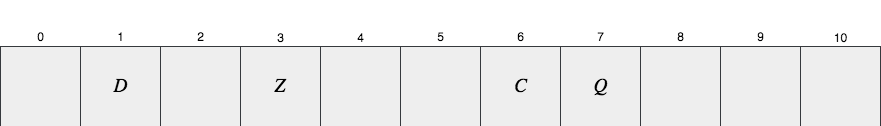
\includegraphics{lookup_table.png}
\end{figure}
  
\section{Array based sequence}

\subsection{Dynamic Array}

\begin{itemize}
	\item Accessor methods
	\begin{itemize}
		\item[] \code{\_\_len\_\_()}
		\item[] \code{\_\_getitem\_\_($k$)}
	\end{itemize}		
	\item Methods
	\begin{itemize}
		\item[] \code{\_make\_array($c$)}
		\item[] \code{append($e$)}
		\item[] \code{\_resize($c$)} 
	\end{itemize}
\end{itemize}

\begin{minted}[bgcolor=LightGray]{python}
class DynamicArray:

    def _make_array(self, c):
        """Return a new array with capacity `c`."""
        return (c * ctypes.py_object)()

    def __init__(self):
        """Create an empty array."""
        self._n = 0                                    
        self._capacity = 1
        self._array = self._make_array(self._capacity) 
    
    def __len__(self):
        """Return the number of element strored in the array."""
        return self._n

    def __getitem__(self, k):
        """Return the element at index `k`."""
        if not 0 <= k < self._n:
            raise IndexError('invalid index')
        return self._array[k]
	
	def __setitem__(self, k, e):
	    """Return the element at index `k`."""
	    self._array[k] = e
	    
	    
	    
	        
    def append(self, e):
        """Add element `e` at the end of the array"""
        if self._n == self._capacity:
            self._resize(2 * self._capacity)
        self._array[self._n] = e
        self._n += 1

    def _resize(self, c):
        """Resize internal array to capacity `c`."""
        B = self._make_array(c)
        for i in range(self._n):
            B[i] = self[i]
        self._capacity = c
        self._array = B
    
    def remove(self, k):
        obj_to_remove = self[k]
        for i in range(k, self._n-1):
            self[i] = self[i+1] 
        self[self._n-1] = None
        self._n -= 1
        return obj_to_remove
    
    def pop(self):
        obj = self[self._n-1]
        self.remove(self._n-1)
        if self._n <= self._capacity / 4:
            self._resize(self._capacity // 2)
        return obj 
        
    def find(self, obj):
        """Return the index of `obj` if `obj` is in the list else `None`"""
        for k in range(self._n):
            if self[k] == obj:
                return k
        return None
        
    def insert(self, obj, k): 
        if not 0 <= k < self._n:
            raise IndexError('invalid index')
        self.append(None)
        for i in range(self._n-1, k, -1):
            self[i] = self[i-1]
        self[k] = obj
\end{minted}
\section{Stack}
A $\bm{Stack}$ is a collection of element that are added and removed according to the \textit{last-in, first-out} principle. Formaly, as stack is an abstract data type characterized by two methods: the method \code{push} and the method \code{pop}. Let $S$ be an instance of a stack. The method \code{push($e$)} adds element $e$ at the top of the stack (usualy at the end?), e.g. if \code{S = [1]} then after executing \code{S.push(2)} we have \code{S = [1, 2]}. The method \code{pop()} remove and return the element at the top of the stack. An instance of a stack also have 3 \textit{accessor methods}: \code{top()} return the element at the top of the stack, \code{is\_empty()} return \code{True} if the stack does not contain any element, and \code{len()} return the number of elements in the stack.

\subsection{Implementing a Stack using a Python List}
\begin{minted}[bgcolor=LightGray]{python}
class ListStack:
    def __init__(self):
        self._data = [] # nonpublic list instance
    
    def __len__(self):
        return len(self._data)
    
    def is_empty(self):
        return len(self._data) == 0
    
    def top(self):
        if self.is_empty():
            return None
        return self._data[-1]
             
    def pop(self):
        if self.is_empty():
            return None 
        return self._data.pop()
            
    def push(self, e):
        self._data.append(e)
\end{minted}

\subsection{implementing a Stack using a Dynamic Array}

\begin{minted}[bgcolor=LightGray]{python}
from dynamic_array import DynamicArray
class ArrayStack:
    def __init__(self):
        self._data = DynamicArray()

    def __len__(self):
        return len(self._data)

    def is_empty(self):
        return len(self._data) == 0
    
    def top(self):
        if self.is_empty():
            return None
        return self._data[-1]

    def pop(self):
        if self.is_empty():
            return None 
        return self._data.pop()

    def push(self, e):
        self._data.append(e)
\end{minted}

\subsection{Example: Evaluation of arithmetic expression}

\section{Queue}
A \textbf{Queue} is a collection of object that are inserted and removed according toe the \textit{first-in, first-out} principle. We usually say that elements enter a queue at the back and are removed from the front. 

\subsection{The ADT Queue}
\begin{itemize}
	\item Methods
	\begin{itemize}
		\item[] \code{enqueue($e$)} Add element $e$ to the end of the queue.
		\item[] \code{dequeue()} Remove and return the first element of the queue.
	\end{itemize}
	\item Accessor methods
	\begin{itemize}
		\item[] \code{\_\_len\_\_()} 
		\item[] \code{is\_empty()}
		\item[] \code{first()} return a reference to the element ar the front of the queue.
	\end{itemize}		
\end{itemize}
\begin{minted}[bgcolor=LightGray]{python}
class Queue:
    
    DEFAILT_CAPACITY = 10
    
    def __init__(self, capacity=DEFAILT_CAPACITY):
        self._data = [None] * capacity
        self._capacity = capacity
        self._size = 0
        self._first = 0

    def __len__(self):
        return self._size

    def is_empty(self):
        return self._size == 0
    
    def first(self):
        if self.is_empty:
            return None
        return self._data[self._first]
        
    def enqueue(self, obj):
        if self._size == self._capacity:
            self._resize(2 * self._capacity)
        avail_idx = (self._first + self._size) % self._capacity
        self._data[avail_idx] = obj
        self._size += 1
        
    def dequeue(self):
        if self.is_empty:
            return None
        obj = self._data[self._first]
        self._data[self._first] = None
        self._first = (self._first + 1) % self._capacity
        self._size -= 1
    	return obj

    def _resize(self, c):
        old_data = self._data
        self._data = [None] * c
        walk = self._first
        for i in range(self._size):
             self._data[i] = old_data[walk]
             walk = (self._first + 1) % self._capacity
        self._front = 0
        self._capacity = c
\end{minted}
An inefficient way to implement a queue would be create an adapter using the Python \code{list}. The method \code{enqueue($e$)} could be implemented with the method \code{append($e$)} and the method \code{dequeue()} could be implementes as follow:
\begin{minted}[bgcolor=LightGray]{python}
class Queue:
    ...
    def dequeue(self):
        if self.is_empty(): return None
        first_obj = self._data[0]
        for i in range(len(self._data)):
            self._data[i] = self._data[i+1]
        self._data[len(self._data)] = None
        self._size -= 1
        return first_obj
\end{minted}

However, this method is tragically inefficient has its time complexity is $\Theta(n)$. Another approach would be to keep an instance variable \code{\_first} to refer to the index of the next element in the queue. When the method \code{dequeue()} is call, the element at index \code{\_first} is replace by \code{Node} and \code{\_first} is increment by one.

\subsection{Using an array circularity}

Suppose the current queue is given by
\[
	\boxx{A}\boxx{B}\boxx{C}\boxx{D}\boxx{E}\boxx{F}\boxx{None}\boxx{None}\boxx{None}\boxx{None}
\]
with a capacity of 10, a size of 6, and index 0 as the first position. Let say we dequeue one time, thus we remove \code{A}, replace it by \code{None} and increment \code{\_first} by one. Now, let's say we enqueue four times for the elements \code{G}, \code{H}, \code{I}, and \code{J}. The resulting queue will look like this

\[
	\boxx{None}\boxx{B}\boxx{C}\boxx{D}\boxx{E}\boxx{F}\boxx{G}\boxx{H}\boxx{I}\boxx{J}
\]

The size is now equal to 9, the first index is 1, and the capacity still 10. Finaly, let say we want to enqueue \code{K}. One option would be to increase the size of the array and insert it at the end. This option call lead to huge waste since decrease and increase often maintaining a modest average size. An other option would be to insert \code{K} at position 0. The arithmetic expression to determine the index of insertion that way is
\[
	\code{\_first} + \code{\_size} \code{\%} \code{\_capacity}
\]
and when we dequeue, instead of incrementing the first index by one, we have to consider the cicularity
\[
\code{\_first} = (\code{\_first} + 1) \code{\%} \code{\_capacity}
\]

\section{Linked list}
\subsection{Singly linked list}
Une liste simplement chaînée est une structure de données concrète constituée
d'une séquence de noeuds à partir d'une référence vers le noeud de tête, où
chaque noeud contient deux références : vers un élément et vers le noeud suivant. On gardera aussi une référence sur le dernier noeud et un entier pour le nombre d'éléments dans la liste.\\

\subsubsection{The Node}
A node contains an element and a pointer to the next node.
\begin{listing}[ht]
	\inputminted[bgcolor=LightGray]{python}{node.py}
	\caption{Singly linked Node}
	\label{listing:singlyLinkedNode}
\end{listing}

Once you have the Node class, you can implement any linked list as follows:
\begin{listing}[ht]
	\inputminted[bgcolor=LightGray]{python}{unit_testing_node.py}
	\caption{Singly linked Node}
	\label{listing:singlyLinkedNode}
\end{listing}

\subsubsection{Interface of a singly linked list}

Now let's write the interface for the class \texttt{SinglyLinkedList}. We define three private variable in the constructor. The instance variables \code{\_head} and \code{\_last} refer to the first and the last element of the list, respectively. The instance variable \code{\_size} is a reference to the last element of the list.     

\begin{itemize}
	\item Methods
	\begin{itemize}
		\item[] \code{append($e$)} Add element $e$ to the end of the list.
		\item[] \code{insert($e$)} Add element $e$ at the beginning of the list
		\item[] \code{remove($k$)} Remove the $k$th element of the list in $O(n)$
	\end{itemize}
	\item Accessor methods
	\begin{itemize}
		\item[] \code{\_\_len\_\_()} return the number of element stored in the list
		\item[] \code{is\_empty()} return \code{True} if the list is empty
		\item[] \code{first()} return a reference to the element at the head of the list.
		\item[] \code{last()} return a reference to the element at the tail of the list.
		\item[] \code{find($e$)} return the index of element $e$ in $O(n)$ or \code{None} 
	\end{itemize}		
\end{itemize}

\begin{listing}[ht]
	\inputminted[bgcolor=LightGray]{python}{singly_linked_list_interface.py}
	\caption{Interface for the singly linked list}
	\label{listing:singly_linked_list_interface}
\end{listing}

We need an \code{append}, an \code{insert}, and a \code{remove} method. The method \code{append} add an element at the end of the liked list. The method \code{insert} add an element at the beginning of the linked list. The method \code{remove} takes an argument \code{k} and remove the element at posistion $k$ in the list.\\ 

The constructor of the singly linked list is
\begin{minted}[bgcolor=LightGray]{python}
class SinglyLinkedList
    def __init__(self):
        self._head = None 
        self._tail = None
        self._size = 0
\end{minted}

\subsubsection{Accessor Methods}
\begin{minted}[bgcolor=LightGray]{python}
class SinglyLinkedList
    ...
    def __len__(self):
        return self._size
    def first(self):
        return self._head.element
    def last(self):
        return self._tail.element
    def find(self, k):
        pass
\end{minted}
The \code{find()} method is more tricky. To be able to reach the $k$th element of a list, we need to move from the head to the tali by going from one node to the other. We will know we reach the tail when a node will refer to None as the nest element. This process is called \textit{traversing} the linked list.
\begin{minted}[bgcolor=LightGray]{python}
class SinglyLinkedList
    ...
    def find(self, e):
        if self.is_empty: 
            return None
        curr = self._head._next
        for i in range(self._size):
            if element == curr: 
                return i
    		curr = curr._next
        return None
\end{minted}

\subsubsection{Insert Methods}
To insert an element at the beginning of the linked list, we first need to check if the list is empty. If not, we need the create a new node with the new element and and instance nest that refer to the current head. After that, we can set the head instance to refer to the new node.
\begin{minted}[bgcolor=LightGray]{python}
class SinglyLinkedList
    ...
    def insert(self, e):
        new_head = Node(e, self._head)
        if self.is_empty():
            self._tail = new_head
        self._head = new_head
        self._size += 1
\end{minted}

\subsubsection{Append Methods}
\begin{minted}[bgcolor=LightGray]{python}
class SinglyLinkedList
    ...
    def append(self, e):
        new_tail = Node(e, None)
        if self.is_empty():
            self._head = new_tail
            self._tail = new_tail
        else:
            self._tail._next = new_tail
            self._tail = new_tail
        self._size += 1
\end{minted}
\subsubsection{Remove Methods}
\begin{minted}[bgcolor=LightGray]{python}
class SinglyLinkedList
    ...
    def remove(self, k):
        if self.is_empty():
            raise EmptyError('the list is empty')
        if not 0 <= k < self._size:
            raise IndexError('index invalid for list of size {}'.format(self._size))
        prev_node = None
        curr_node = self._head
        for i in range(k):
            prev_node = curr_node        # curr_node is index `k-1`
            curr_node = curr_node._next  # curr_node is index `k`
        if prev_node is None:            # index `k` is 0
            self._head = curr_node._next # remove current head
        else:
            prev_node._next = curr_node._next # remove current node
        self._size -= 1
        if self._size == 0:             
            self._tail = None           # remove reference tail <- removed node 
        if prev_node._next is None:     # tail was removed	
            self._tail = prev_node
        return curr_node._element
\end{minted}

\section{The Doubly linked List}

The node of a doubly linked list have 3 instances: \code{element} is a reference to the value stored, \code{prev} is a reference to the previous element, and \code{next} is a reference to the next element. 
\begin{minted}[bgcolor=LightGray]{python}
class Node:
    def __init__(self, element, prev, next):
        self.element = element
        self.prev = prev
        self.next = next
\end{minted}

A doubly linked list have 2 special nodes instance at the beginning and the end of the list: the \textbf{header} node have a reference to the first element of the list and the \textbf{trailer} node have a reference to the last element of the list stored in is \code{prev} instance.

\begin{minted}[bgcolor=LightGray]{python}
class DoublyLinkedList:
    class _Node:
       ...
    def __init__(self):
        self._header = self._Node(None, None, None)
        self._trailer = self._Node(None, None, None)
        self._header.next = self._trailer
        self._trailer.prev = self._header
        self._size = 0
\end{minted}

\subsection{Methods}
\begin{itemize}
	\item Methods
	\begin{itemize}
		\item[] \code{append($e$)} Add element $e$ to the end of the list in $O(1)$.
		\item[] \code{insert($e$)} Add element $e$ at the beginning of the list in $O(1)$
		\item[] \code{remove($k$)} Remove the $k$th element of the list in $O(?)$
		\item[] \code{insert\_between($e$, prev, next)}
	\end{itemize}
	\item Accessor methods
	\begin{itemize}
		\item[] \code{\_\_len\_\_()} return the number of element stored in the list
		\item[] \code{is\_empty()} return \code{True} if the list is empty
		\item[] \code{first()} return a reference to the element at the head of the list in $O(1)$.
		\item[] \code{last()} return a reference to the element at the beginning of the list in $O(1)$.
		\item[] \code{find($e$)} return the index of element $e$ in $O(n)$ or \code{None} 
	\end{itemize}		
\end{itemize}

\begin{minted}[bgcolor=LightGray]{python}
class DoublyLinkedList:
    ...
    def __len__(self):
        return self._size
    def is_empty(self):
        return self._size == 0
    def first(self):
        if self.is_empty():
            raise EmptyError('the list is empty')
        return self._header.next.element
    def last(self):
        if self.is_empty():
            raise EmptyError('the list is empty')
        return self._trailer.prev.element
    def find(self, e):
        if self.is_empty():
            raise EmptyError('the list is empty')
        curr_node = self._header.next
        for i in range(self._size):
            if element == curr_node:
                return i
            curr_node = curr_node._next
        return None
\end{minted}

\begin{minted}[bgcolor=LightGray]{python}
class DoublyLinkedList:
    ...
    def append(e):
        new_node = self._Node(e, self._trailer.prev, self._trailer)
        self._trailer.prev.next = new_node
        self._trailer.prev = new_node
        self._size += 1
        
    def insert(self, element):
        new_node = self._Node(e, self._header, self._header.next)
        self._header.next.prev = new_node
        self._header.next = new_node
        self._siz += 1
    
    def remove(self, k):
        if self.is_empty():
            return EmptyError('list is empty')
        if not 0 <= k < self._size:
            return IndexError('index out of bound')
        curr_node = self._header.next
        for i in range(k):
            curr_node = curr_node.next
        curr_node.prev.next = curr_node.next
        curr_node.next.prev = curr_node.prev
        self._size -= 1
        curr_node.next = None
        return curr_node.element
        
    def insert_between(self, e, k1, k2):
        curr = self._header.next
        for i in range(k1):
            curr = curr.next
        new = self._Node(e, curr, curr.next)
        curr.next.prev = new
        curr.next = new
        self._size += 1
\end{minted}

\section{Double Ended Queue}


\section{The Positional List}


\section{Tree}

\begin{minted}[bgcolor=LightGray]{python}
from ListQueue import ListQueue

class DoublyLinkedList:
...
def __len__(self):
return self._size
def is_empty(self):
return self._size == 0
def first(self):
if self.is_empty():
raise EmptyError('the list is empty')
return self._header.next.element
def last(self):
if self.is_empty():
raise EmptyError('the list is empty')
return self._trailer.prev.element
def find(self, e):
if self.is_empty():
raise EmptyError('the list is empty')
curr_node = self._header.next
for i in range(self._size):
if element == curr_node:
return i
curr_node = curr_node._next
return None
\end{minted}

\begin{minted}[bgcolor=LightGray]{python}
def _link_leaves(self):
    Q = ListQueue()
    found_first_leaf = False
    prev_leaf = None
    
    Q.enqueue(self._root)
    
    while not Q.is_empty():
        p = Q.dequeue()
        if prev_leaf is not None and p._is_leaf():
            prev_leaf._right_leaf = p
            prev_leaf = p
        if not found_first_leaf and p._is_leaf():
            self._first_leaf = p
            prev_leaf = self._first_leaf
        for c in p._children():
            Q.enqueue(c)
    self._last_leaf = p
    self._last_leaf._right_leaf = self._first_leaf
    
\end{minted}

\begin{minted}[bgcolor=LightGray]{python}
def find_int(S, k, i, j):
    if S[i] + S[j] 
\end{minted}

\begin{minted}[bgcolor=LightGray]{python}

\end{minted}






\end{document}
